\section{Additional experiments}
\label{sec:additional}
After successfully reproducing most of the experiments, we thought of some interesting extensions. Specifically, we investigated the choice of sampling hyperparameters $\epsilon$ and $T$, annealing schedule and network architecture, which we identified as important but unexplored in the original work. \vspace{-0.9mm}

\subsection{Sensitivity on sampling parameters}
The authors report the interval $\epsilon \in (5\cdot 10^{-6}, 5\cdot 10^{-5})$ and $T = 100$ as robust hyperparameters for sampling. Motivated by sensitivity to $\epsilon$ in the toy examples, we investigate these hyperparameters in more detail on real data from the CIFAR-10 dataset. We sampled with a smaller $\epsilon$ (\autoref{fig:1e-6eps}) and a larger $\epsilon$ (\autoref{fig:1e-1eps}), where the former yielded only noise since the step was not large enough to move away from the noisy initial point, and the latter resulted in samples being one-coloured because too large step size escaped allowed pixel values and was artificially clipped to the endpoints of pixel intervals. Similarly, a large $T$ results in smoother images (\autoref{fig:t-1000}), but with much fewer details, probably due to convergence to a local mode representing some kind of generic class image, and a small $T$ (\autoref{fig:t-10}) being mostly noise with only slightly distinguishable shapes. While the reasoning here is speculative, we here would like to emphasise the sensitivity to choice of $\epsilon$ and $T$, as already seen in the toy GMM experiment in \autoref{sec:repr-of-toy}. A suggested future work might concern different annealing strategies where $\epsilon$ or $T$ could be adjusted for different noise levels.\vspace{-2mm}

\begin{figure}[h!]
    \centering
    \subfloat[$\epsilon=10^{-6}, T=100$]{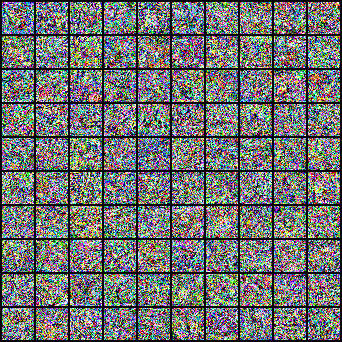
\includegraphics[width=0.24\linewidth]{figures/samples/samples_eps/1e-6.png}\label{fig:1e-6eps}}\hspace{1mm}
    \subfloat[$\epsilon=10^{-1}, T=100$]{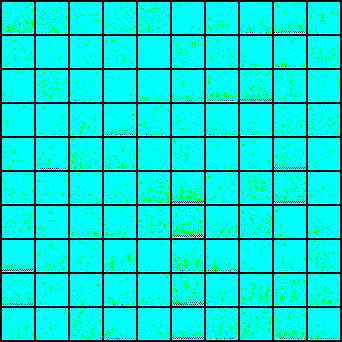
\includegraphics[width=0.24\linewidth]{figures/samples/samples_eps/1e-1.png}\label{fig:1e-1eps}}\hspace{1mm}
    \subfloat[$\epsilon=2\cdot 10^{-5}, T=10$]{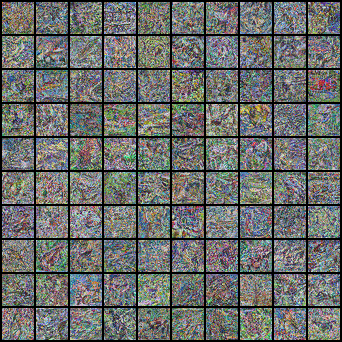
\includegraphics[width=0.24\linewidth]{figures/samples/samples_T/refinenet128_cifar10_L10_step120000_t10.png}\label{fig:t-10}}\hspace{1mm}
    \subfloat[$\epsilon=2\cdot 10^{-5}, T=10^3$]{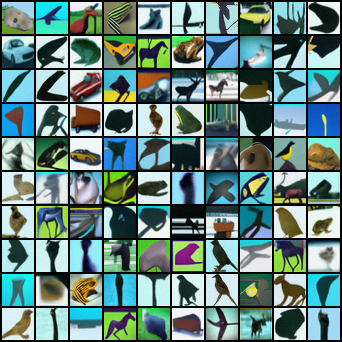
\includegraphics[width=0.24\linewidth]{figures/samples/samples_T/refinenet128_cifar10_L10_step120000_t1000.png}\label{fig:t-1000}}
     \caption{Samples from the best CIFAR-10 model with different values of $\epsilon$ and $T$.}
     \label{fig:varying-epsilon}
\end{figure}
% Considering that the step size of the annealed Langevin dynamic is proportional to the hyperparameter $\epsilon$, we can expect the behaviour observed in Figure \ref{fig:varying-epsilon}. If $\epsilon$ is too small, the image takes too small steps towards high density regions, and therefore never reaches them, remaining noisy. On the other hand, if the value of $\epsilon$ is too large, we speculate that the images converge to predominant modes that probably have large support.
 
\subsection{Linear annealing schedule}
We also train a model with linear annealing schedule instead of geometric on CIFAR-10 dataset. We hypothesise that geometric annealing might be too aggressive in the sense that most of noise values are low, which results in fine-tuning edges without capturing global features first. This is manifested in some samples being smooth, but not having a distinct shape of any reasonable object. From visual inspection of the results (\autoref{fig:linear}) we can see that intuition was correct, as these samples capture much more detail and complexity than with geometric annealing (\autoref{fig:cifar10-samp}). However, the images are visibly more noisy. We can explain this tendency using the inverse of the previous logic, namely that there are not enough noise levels in the low spectrum of values, thus precluding the sampling of sharper images. We believe some combination of these annealing schedules could solve this issue and result in very good samples, but also add to the complexity of the model.\vspace{-3mm}

\begin{figure}[h!]
    \centering
    \subfloat[50k iterations]{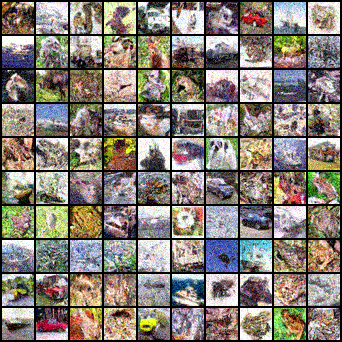
\includegraphics[width=0.24\linewidth]{figures/samples/linear/linear-50k.png}\label{fig:linear-50k}}\hspace{1mm}
    \subfloat[100k iterations]{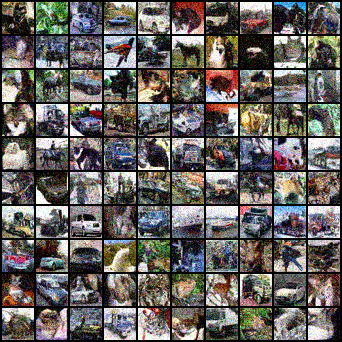
\includegraphics[width=0.24\linewidth]{figures/samples/linear/linear-100k.png}\label{fig:linear-100k}}\hspace{1mm}
    \subfloat[150k iterations]{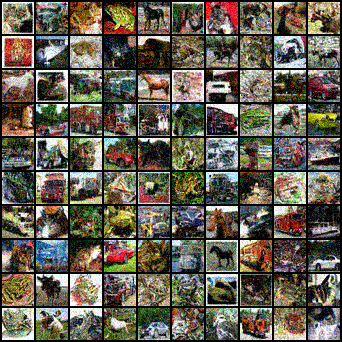
\includegraphics[width=0.24\linewidth]{figures/samples/linear/linear-150k.png}\label{fig:linear-150k}}\hspace{1mm}
    \subfloat[200k iterations]{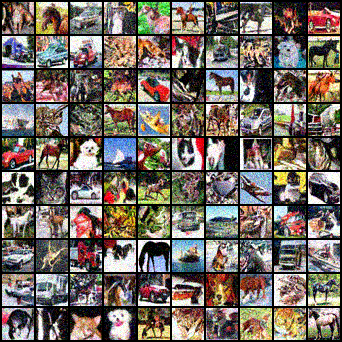
\includegraphics[width=0.24\linewidth]{figures/samples/linear/linear-200k.png}\label{fig:linear-200k}}
     \caption{Samples from model trained on CIFAR-10 with linear annealing schedule.}
     \label{fig:linear}
     \vspace{-3mm}
\end{figure}

\subsection{Different architecture of the score network}
The authors emphasise the choice of network architecture as important role and leave experimenting with different designs as future work. We address this by replacing the U-Net structure with the ResNet from the toy example in \autoref{sec:repr-of-toy} on CIFAR-10, but to avoid changing the architecture too much, we add conditional instance normalisation and dilated convolutions, as well as multiplying the number of filters by factor of 4 in each block to match the number of parameters in the RefineNet. Here we can only conclude that this simple architecture did not result in meaningful samples and that the choice of structure seems to be important. We believe the main reason for these subpar results is lack of skip connections as in U-Net type architectures. We also acknowledge that training hyperparameters would have to be tuned for this network to meaningfully compare the results. However, when taken in combination with the results from the main experiments in \autoref{sec:main-exp}, and assuming that our hypothesis -- that minor differences in RefineNet architecture between our implementation and the one from the original paper contribute to significantly worse performance in terms of FID score -- is correct, this would suggest that the method is perhaps overly reliant on architectural details. We suggest that more investigation is needed to determine exactly which aspects of the score network architecture are crucial for good performance.

\begin{figure}[H]
    \centering
    \subfloat[100k iterations]{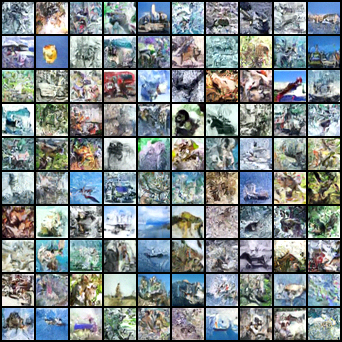
\includegraphics[width=0.31\linewidth]{figures/samples/resnet_100k.png}\label{fig:resnet-100k}}\hspace{1mm}
    \subfloat[150k iterations]{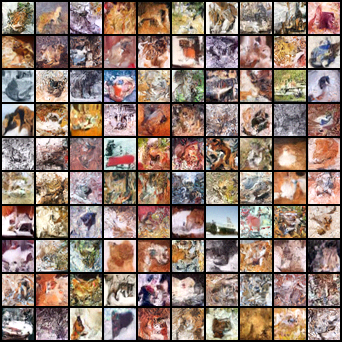
\includegraphics[width=0.31\linewidth]{figures/samples/resnet_150k.png}\label{fig:resnet-150k}}\hspace{1mm}
    \subfloat[200k iterations]{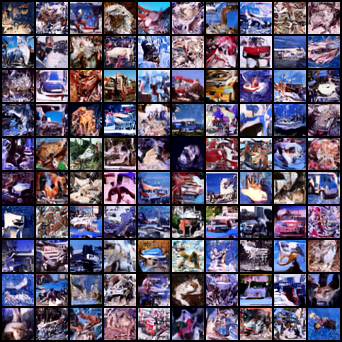
\includegraphics[width=0.31\linewidth]{figures/samples/resnet_200k.png}\label{fig:resnet-200k}}
     \caption{Samples from a ResNet model trained on CIFAR-10.}
     \label{fig:resnet}
\end{figure}